\documentclass[11pt]{report}


\usepackage{
        outline,
        pmgraph,
        graphicx,
        verbatim,
        hyperref,
        enumitem,
        float,
        amsmath,
        xcolor,
        listings,
        xparse,
        hyperref,
        booktabs,
}
\hypersetup{
    linkcolor=blue,
    colorlinks=true,
    urlcolor=blue,
    linkbordercolor = {white},
}
\definecolor{codegreen}{rgb}{0,0.6,0}
\definecolor{codegray}{rgb}{0.5,0.5,0.5}
\definecolor{codepurple}{rgb}{0.58,0,0.82}
\definecolor{backcolour}{rgb}{0.95,0.95,0.92}

\lstdefinestyle{mystyle}{
    backgroundcolor=\color{backcolour},   
    commentstyle=\color{codegreen},
    keywordstyle=\color{magenta},
    numberstyle=\tiny\color{codegray},
    stringstyle=\color{codepurple},
    basicstyle=\ttfamily\footnotesize,
    breakatwhitespace=false,         
    breaklines=true,                 
    captionpos=b,                    
    keepspaces=true,                 
    numbersep=5pt,                  
    showspaces=false,                
    showstringspaces=false,
    showtabs=false,                  
    tabsize=2
}

\lstset{style=mystyle}

\NewDocumentCommand{\codeword}{v}{%
    \texttt{\textcolor{black}{#1}}%
}

\NewDocumentCommand{\linkword}{v}{%
    \texttt{\textcolor{blue}{#1}}%
}
\setlength{\parindent}{0pt} 

\usepackage[normalem]{ulem}

\title{
    
\includegraphics[width=3in]{assets/up.png} \\
    \vspace*{1in}
    \textbf{Machine Project 1}
}


\author{Aaron Paul Gapud\\
        Brymer Bernard Meneses\\
		\vspace*{0.5in} \\
		College of Science\\
        \textbf{University of the Philippines - Baguio}\\
        Gov. Pack Road, Baguio City, Baguio 2600
       } \date{\today}

\setlength{\oddsidemargin}{0in} \setlength{\evensidemargin}{0in}
\setlength{\topmargin}{0in}     \setlength{\headsep}{-.25in}
\setlength{\textwidth}{6.5in}   \setlength{\textheight}{8.5in}

\setlength{\parindent}{0pt}

\renewcommand\thesection{\Alph{section}.} 
\renewcommand\thesubsection{\Roman{subsection}.} 

\date{}

\renewcommand*\contentsname{Table of Contents}

\begin{document}
\maketitle 
\tableofcontents
\newpage


\section{Introduction}

\emph{Ghostless Pacman} is a 2021 adaptation of the video game series Pac-man™,
only without the ghosts. It was mainly created using the C Programming
language by Brymer Meneses and Paul Gapud, Computer Science freshmen
from the University of the Philippines -- Baguio.


\section{Description}

The program mainly utilized the concept of arrays to return a working 10-by-10
game board. To improve user experience, visual and audio elements were added to
the program interface. This feature is the significant purpose of using a
resource called \emph{SDL} or \href{https://www.libsdl.org/}{Simple DirectMedia Layer},
to render animation, play sound, and showcase creatives.

\begin{table}[H]
    \centering
    \def\arraystretch{2.5}
    \begin{tabular}{ c c c }
        \toprule
        Instruction & Definition & Representation \\
        \midrule
        O & Pacman & 
\includegraphics[scale=0.1]{assets/pacman_sample.png} \\
        $*$ & Food & 
\includegraphics[scale=0.1]{assets/food_sample.png} \\
        X & Blocks & 
\includegraphics[scale=0.1]{assets/block_sample.png} \\
        \$ & Door & 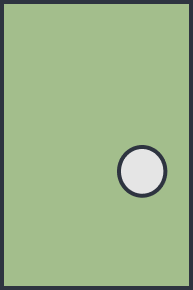
\includegraphics[scale=0.1]{assets/door_sample.png}\\
        \bottomrule
    \end{tabular}
    \caption{The visual representation of symbols in the Ghostless Pacman game}
    \label{tab:1}
\end{table}

Pacman, instead of a a plain `O' might definitely look more like Pacman. In
fact, this Pacman actually munches. Rendering its animation is a feature of the
said SDL library. The same feature allowed the program to display food pieces
as something more delicious than asterisks or any other punctuation, that is,
cherries. The game obstacles that look tougher than `X', and instead of a
dollar sign for the exit door, an exit door.\\

More than these, the resource is also used to render other images such as the
overall interface of the game, including the menus, prompts, and warnings.
Visual assets have been originally constructed using an online software called
\href{https://www.figma.com/}{Figma}.\\

Another use of SDL is for the incorporation of sounds and music into the game.
The audio assets used in the game are royalty-free and, if whose owner demands
copyright, are given proper credit in About the Game.\\

In terms of functions, below are some that have been integrated into the
program as the project requires:

\begin{enumerate}
    \item \codeword{fill_board_with_foods}\\
    \hspace{1em} This function will randomly fill the board with foods
    \item \codeword{fill_board_with_blocks}\\
    \hspace{1em} This function will randomly fill the board with blocks
    \item \codeword{check_if_player_won} and \codeword{check_player_status}\\
    \hspace{1em} These functions work hand-in-hand to check if the player reaches the exit sign after eating all the food pieces,
    or otherwise displays the player status of whether he or she wins or loses
\end{enumerate}

Another crucial function defined is
\codeword{check_for_impossible_win_scenario}, which checks and ensures that any
round in the game is winnable by preventing
\codeword{impassable_adjacent_neighbors}, that is, no food piece or exit door
is surrounded by blocks from all sides.\\

The code also made use of header (.h) files to declare certain variables for
the game. Some major concepts involved are for and while loops, structs, and
switch cases.

\\
\\
Throughout the documentation of the code, the following definitions explain
some of the terms that will be encountered:

\begin{description}
    \item[state]{is a certain condition of something (e.g., state of the game, state of the player)}
    \item[sprite]{is a computer graphic which can move and perform actions on screen}
    \item[asset]{is anything that is incorporated into a video game, such as characters, objects, and sound effects}
    \item[pointer]{(in programming) is an object that stores and references a memory address in the computer}
    \item[struct]{is a composite data type declaration that groups variables under one name in memory, accessible via a single pointer} 
    \item[anti-aliasing]{(in computer graphics) is the removing of jagged edges in an image rendered using pixels}
\end{description}

\section{Algorithm}
\subsection{Pre-game Algorithm}

\begin{enumerate}
    \item Application launches
    \begin{enumerate}[label=\alph*.]
        \item
            \begin{itemize}[label={}]
                \item If the user presses 1, the \emph{Start} option will be highlighted
                \item \hspace{1cm} If the user presses Enter, proceed to Step 3
            \end{itemize}
        \item 
            \begin{itemize}[label={}]
                \item If the user presses 2, the \emph{Tutorial} option will be highlighted
                \item \hspace{1cm} the user presses Enter, proceed to Step 4
            \end{itemize}
        \item 
            \begin{itemize}[label={}]
                \item  If the user presses 3, the \emph{Exit} option will be highlighted
                \item \hspace{1cm} If the user presses Enter, proceed to Step 5
            \end{itemize}
        \item 
            \begin{itemize}[label={}]
                \item  If the user presses A, the \emph{About the Game} option will be highlighted
                \item \hspace{1cm} If the user presses Enter, proceed to Step 3
            \end{itemize}
        
        \item Else, display a wrong input reminder.
    \end{enumerate}
    
    \item User chooses from the menu options:
        \begin{enumerate}[label=\alph*]
            \item
            \begin{itemize}[label={}]
                \item If the user input is from 2 to 9, display chosen number 
                \item \hspace{1cm} If the user presses Enter, proceed to In-play Algorithm
            \end{itemize}
            \item  If the user presses M, go back to Step 2
	        \item Else, display a wrong input reminder
        \end{enumerate}
    \item User chooses the number of food pieces s/he wants for the game
        \begin{enumerate}[label=\alph*]
            \item User chooses the number of food pieces s/he wants for the game
            \begin{itemize}[label={}]
                \item If the user input is from 2 to 9, display chosen number
            \end{itemize}
            \item If the user presses Enter, proceed to In-play Algorithm
            \item If the user presses M, go back to Step 2
            \item Else, display a wrong input reminder
        \end{enumerate}
    \item Program shows the first slide of the Tutorial
        \begin{enumerate}[label=\alph*]
        \item User navigates through the slides by pressing arrow left (←) and arrow right (→)
        \item If the user presses M, go back to Step 2
        \item If the user presses 1, proceed to Step 3
        \item If the user presses X, proceed to Step 5
        \item Else, display a wrong input reminder
        \end{enumerate}
    \item Program prompts a quit window
        \begin{enumerate}[label=\alph*]
            \item If the user presses Y, exit the program
            \item If the user presses N, the prompt closes
        \end{enumerate}
\end{enumerate}


\subsection{In-game Algorithm}

\begin{enumerate}
    \item Display a 10-by-10 board, with Pacman on the top left, the food
        pieces based on the accepted user input, the randomly distributed
        blocks, and the randomly placed exit door
        \begin{enumerate}[label=\alph*]
            \item If the user presses W, pacman moves up
            \item If the user presses S, pacman moves down
            \item If the user presses A, pacman moves left
            \item If the user presses D, pacman moves right
            \item If the user presses M, the program goes back to menu (go back to Step 2 of the Pre-play Algorithm)
            \item If the user presses X, the program prompts a quit window (recall Step 5 of the Pre-play Algorithm)
            \begin{itemize}[label={}]
                \item If the user presses Y, exit the program
                \item If the user presses N, the prompt closes
            \end{itemize}
        \end{enumerate}
    \item User plays the game by moving Pacman to eat the food pieces towards the exit door
        \begin{enumerate}[label=\alph*]
            \item If Pacman hits a block, display a Game Over prompt
            \item If Pacman gets out of the board, display a Game Over prompt
            \item If Pacman reaches the door without eating all the food pieces, display a Game Over prompt
            \item If Pacman reaches the door after eating all the food pieces, display a Game Victory prompt
        \end{enumerate}
    \item With the prompts from the game results, the user chooses between the options to restart, return to menu, or exit the game
        \begin{enumerate}[label=\alph*]
            \item If the user presses R, restart the game (go back to Step 3 of the Pre-play Algorithm)
            \item If the user presses M, return to menu (go back to Step 2 of the Pre-play Algorithm)
            \item If the user presses X, the program prompts a quit window (recall Step 5 of the Pre-play Algorithm)
                \begin{itemize}[label={}]
                    \item If the user presses Y, exit the program
                    \item If the user presses N, the prompt closes
                \end{itemize}
            \item Else, display a wrong input reminder
        \end{enumerate}
\end{enumerate}


\section{Error handling}

As seen in the algorithms, the game was programmed to handle errors of user input by displaying wrong input reminders per various instances. To recall, below is a list of these occurrences:\\
    \begin{itemize}[label={}]
        \item In Menu, the program displays a reminder when the user keypress is not '1', '2', '3', or 'A'
        \item In the Game
            \begin{itemize}[label={}]
                \item In choosing the food number, the program displays a reminder when the user chooses a number outside the range from 2 to 9
                \item In playing the game, the program displays a reminder when the user presses keys other than 'W', 'S', 'A', or 'D' to move Pacman, and when the user presses keys other than 'M' to return to menu or 'X' to exit the game
                \item In choosing an option after the game results, displayed through the game prompts, the program displays a reminder when the user presses keys other than 'R' to restart, 'M' to return to menu, or 'X' to exit
            \end{itemize}
        \item In Tutorial
            \begin{itemize}[label={}]
                \item In navigating, the program displays a reminder when the user presses keys other than '←' or '→' to navigate through the tutorial slides, when the user presses keys other than 'M' to return to menu
                \item In the last slide, the program displays a reminder when the user presses keys other than '1' to start the game, 'M' to return to menu, or 'X' to exit
            \end{itemize}
        \item In About the Game, the program displays a reminder when the user presses keys other than 'M' to return to menu
    \end{itemize}
\documentclass[11pt]{report}


\usepackage{
        outline,
        pmgraph,
        graphicx,
        verbatim,
        hyperref,
        enumitem,
        float,
        amsmath,
        xcolor,
        listings,
        xparse,
        hyperref
}

\definecolor{codegreen}{rgb}{0,0.6,0}
\definecolor{codegray}{rgb}{0.5,0.5,0.5}
\definecolor{codepurple}{rgb}{0.58,0,0.82}
\definecolor{backcolour}{rgb}{0.95,0.95,0.92}

\lstdefinestyle{mystyle}{
    backgroundcolor=\color{backcolour},   
    commentstyle=\color{codegreen},
    keywordstyle=\color{magenta},
    numberstyle=\tiny\color{codegray},
    stringstyle=\color{codepurple},
    basicstyle=\ttfamily\footnotesize,
    breakatwhitespace=false,         
    breaklines=true,                 
    captionpos=b,                    
    keepspaces=true,                 
    numbersep=5pt,                  
    showspaces=false,                
    showstringspaces=false,
    showtabs=false,                  
    tabsize=2
}

\lstset{style=mystyle}

\NewDocumentCommand{\codeword}{v}{%
    \texttt{\textcolor{black}{#1}}%
}
\setlength{\parindent}{0pt} 

\usepackage[normalem]{ulem}

\title{
    
\includegraphics[width=3in]{upbag.png} \\
    \vspace*{1in}
    \textbf{Machine Project 1}
}


\author{Aaron Paul Gapud\\
        Brymer Bernard Meneses\\
		\vspace*{0.5in} \\
		College of Science\\
        \textbf{University of the Philippines - Baguio}\\
        Gov. Pack Road, Baguio City, Baguio 2600
       } \date{\today}

\setlength{\oddsidemargin}{0in} \setlength{\evensidemargin}{0in}
\setlength{\topmargin}{0in}     \setlength{\headsep}{-.25in}
\setlength{\textwidth}{6.5in}   \setlength{\textheight}{8.5in}

\setlength{\parindent}{0pt}

\renewcommand\thesection{\Alph{section}.} 
\renewcommand\thesubsection{\Roman{subsection}.} 

\date{}

\renewcommand*\contentsname{Table of Contents}

\begin{document}
\maketitle 
\tableofcontents
\newpage


\section{Introduction}

\emph{Ghostless Pacman} is a 2021 adaptation of the video game series Pac-man™,
only without the, as stated, ghosts. It was mainly recreated using the C
language by Brymer Meneses and Paul Gapud, Computer Science freshmen
from the University of the Philippines - Baguio.


\section{Description}

The program mainly utilized the concept of arrays to return a working 10-by-10
game board. To improve user experience, visual and audio elements were added to
the program interface. This feature is the significant purpose of using a
resource called \emph{SDL} or \href{https://www.libsdl.org/}{Simple DirectMedia Layer},
to render animation, play sound, and showcase creatives.

\begin{table}[H]
    \centering
    \def\arraystretch{2.5}
    \begin{tabular}{ c c c }
        \toprule
        Instruction & Definition & Representation \\
        \midrule
        O & Pacman & 
\includegraphics[scale=0.1]{assets/pacman_sample.png} \\
        $*$ & Food & 
\includegraphics[scale=0.1]{assets/food_sample.png} \\
        X & Blocks & 
\includegraphics[scale=0.1]{assets/block_sample.png} \\
        \$ & Door & 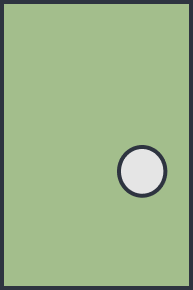
\includegraphics[scale=0.1]{assets/door_sample.png}\\
        \bottomrule
    \end{tabular}
    \caption{The visual representation of symbols in the Ghostless Pacman game}
    \label{tab:1}
\end{table}

Pacman, instead of a a plain `O' might definitely look more like Pacman. In
fact, this Pacman actually munches. Rendering its animation is a feature of the
said SDL library. The same feature allowed the program to display food pieces
as something more delicious than asterisks or any other punctuation, that is,
cherries. The game obstacles that look tougher than `X', and instead of a
dollar sign for the exit door, an exit door.\\

More than these, the resource is also used to render other images such as the
overall interface of the game, including the menus, prompts, and warnings.
Visual assets have been originally constructed using an online software called
\href{https://www.figma.com/}{Figma}.\\

Another use of SDL is for the incorporation of sounds and music into the game.
The audio assets used in the game are royalty-free and, if whose owner demands
copyright, are given proper credit in About the Game.\\

In terms of functions, below are some that have been integrated into the
program as the project requires:

\begin{enumerate}
    \item \codeword{fill_board_with_foods}\\
    \hspace{1em} This function will randomly fill the board with foods
    \item \codeword{fill_board_with_blocks}\\
    \hspace{1em} This function will randomly fill the board with blocks
    \item \codeword{check_if_player_won} and \codeword{check_player_status}\\
    \hspace{1em} These functions work hand-in-hand to check if the player reaches the exit sign after eating all the food pieces,
    or otherwise displays the player status of whether he or she wins or loses
\end{enumerate}

Another crucial function defined is
\codeword{check_for_impossible_win_scenario}, which checks and ensures that any
round in the game is winnable by preventing
\codeword{impassable_adjacent_neighbors}, that is, no food piece or exit door
is surrounded by blocks from all sides.\\

The code also made use of header (.h) files to declare certain variables for
the game. Some major concepts involved are for and while loops, structs, and
switch cases.

\section{Algorithm}
\subsection{Pre-game Algorithm}

\begin{enumerate}
    \item Application launches
    \begin{enumerate}[label=\alph*.]
        \item
            \begin{itemize}[label={}]
                \item If the user presses 1, the \emph{Start} option will be highlighted
                \item \hspace{1cm} If the user presses Enter, proceed to Step 3
            \end{itemize}
        \item 
            \begin{itemize}[label={}]
                \item If the user presses 2, the \emph{Tutorial} option will be highlighted
                \item \hspace{1cm} the user presses Enter, proceed to Step 4
            \end{itemize}
        \item 
            \begin{itemize}[label={}]
                \item  If the user presses 3, the \emph{Exit} option will be highlighted
                \item \hspace{1cm} If the user presses Enter, proceed to Step 5
            \end{itemize}
        \item 
            \begin{itemize}[label={}]
                \item  If the user presses A, the \emph{About the Game} option will be highlighted
                \item \hspace{1cm} If the user presses Enter, proceed to Step 3
            \end{itemize}
        
        \item Else, display a wrong input reminder.
    \end{enumerate}
    
    \item User chooses from the menu options:
        \begin{enumerate}[label=\alph*]
            \item
            \begin{itemize}[label={}]
                \item If the user input is from 2 to 9, display chosen number 
                \item \hspace{1cm} If the user presses Enter, proceed to In-play Algorithm
            \end{itemize}
            \item  If the user presses M, go back to Step 2
	        \item Else, display a wrong input reminder
        \end{enumerate}
    \item User chooses the number of food pieces s/he wants for the game
        \begin{enumerate}[label=\alph*]
            \item User chooses the number of food pieces s/he wants for the game
            \begin{itemize}[label={}]
                \item If the user input is from 2 to 9, display chosen number
            \end{itemize}
            \item If the user presses Enter, proceed to In-play Algorithm
            \item If the user presses M, go back to Step 2
            \item Else, display a wrong input reminder
        \end{enumerate}
    \item Program shows the first slide of the Tutorial
        \begin{enumerate}[label=\alph*]
        \item User navigates through the slides by pressing arrow left (←) and arrow right (→)
        \item If the user presses M, go back to Step 2
        \item If the user presses 1, proceed to Step 3
        \item If the user presses X, proceed to Step 5
        \item Else, display a wrong input reminder
        \end{enumerate}
    \item Program prompts a quit window
        \begin{enumerate}[label=\alph*]
            \item If the user presses Y, exit the program
            \item If the user presses N, the prompt closes
        \end{enumerate}
\end{enumerate}


\subsection{In-game Algorithm}

\begin{enumerate}
    \item Display a 10-by-10 board, with Pacman on the top left, the food
        pieces based on the accepted user input, the randomly distributed
        blocks, and the randomly placed exit door
        \begin{enumerate}[label=\alph*]
            \item If the user presses W, pacman moves up
            \item If the user presses S, pacman moves down
            \item If the user presses A, pacman moves left
            \item If the user presses D, pacman moves right
            \item If the user presses M, the program goes back to menu (go back to Step 2 of the Pre-play Algorithm)
            \item If the user presses X, the program prompts a quit window (recall Step 5 of the Pre-play Algorithm)
            \begin{itemize}[label={}]
                \item If the user presses Y, exit the program
                \item If the user presses N, the prompt closes
            \end{itemize}
        \end{enumerate}
    \item User plays the game by moving Pacman to eat the food pieces towards the exit door
        \begin{enumerate}[label=\alph*]
            \item If Pacman hits a block, display a Game Over prompt
            \item If Pacman gets out of the board, display a Game Over prompt
            \item If Pacman reaches the door without eating all the food pieces, display a Game Over prompt
            \item If Pacman reaches the door after eating all the food pieces, display a Game Victory prompt
        \end{enumerate}
    \item With the prompts from the game results, the user chooses between the options to restart, return to menu, or exit the game
        \begin{enumerate}[label=\alph*]
            \item If the user presses R, restart the game (go back to Step 3 of the Pre-play Algorithm)
            \item If the user presses M, return to menu (go back to Step 2 of the Pre-play Algorithm)
            \item If the user presses X, the program prompts a quit window (recall Step 5 of the Pre-play Algorithm)
                \begin{itemize}[label={}]
                    \item If the user presses Y, exit the program
                    \item If the user presses N, the prompt closes
                \end{itemize}
            \item Else, display a wrong input reminder
        \end{enumerate}
\end{enumerate}


\section{Error handling}

As seen in the algorithms, the game was programmed to handle errors of user input by displaying wrong input reminders per various instances. To recall, below is a list of these occurrences:\\
    \begin{itemize}[label={}]
        \item In Menu, the program displays a reminder when the user keypress is not '1', '2', '3', or 'A'
        \item In the Game
            \begin{itemize}[label={}]
                \item In choosing the food number, the program displays a reminder when the user chooses a number outside the range from 2 to 9
                \item In playing the game, the program displays a reminder when the user presses keys other than 'W', 'S', 'A', or 'D' to move Pacman, and when the user presses keys other than 'M' to return to menu or 'X' to exit the game
                \item In choosing an option after the game results, displayed through the game prompts, the program displays a reminder when the user presses keys other than 'R' to restart, 'M' to return to menu, or 'X' to exit
            \end{itemize}
        \item In Tutorial
            \begin{itemize}[label={}]
                \item In navigating, the program displays a reminder when the user presses keys other than '←' or '→' to navigate through the tutorial slides, when the user presses keys other than 'M' to return to menu
                \item In the last slide, the program displays a reminder when the user presses keys other than '1' to start the game, 'M' to return to menu, or 'X' to exit
            \end{itemize}
        \item In About the Game, the program displays a reminder when the user presses keys other than 'M' to return to menu
    \end{itemize}
\documentclass[11pt]{report}


\usepackage{
        outline,
        pmgraph,
        graphicx,
        verbatim,
        hyperref,
        enumitem,
        float,
        amsmath,
        xcolor,
        listings,
        xparse,
        hyperref
}

\definecolor{codegreen}{rgb}{0,0.6,0}
\definecolor{codegray}{rgb}{0.5,0.5,0.5}
\definecolor{codepurple}{rgb}{0.58,0,0.82}
\definecolor{backcolour}{rgb}{0.95,0.95,0.92}

\lstdefinestyle{mystyle}{
    backgroundcolor=\color{backcolour},   
    commentstyle=\color{codegreen},
    keywordstyle=\color{magenta},
    numberstyle=\tiny\color{codegray},
    stringstyle=\color{codepurple},
    basicstyle=\ttfamily\footnotesize,
    breakatwhitespace=false,         
    breaklines=true,                 
    captionpos=b,                    
    keepspaces=true,                 
    numbersep=5pt,                  
    showspaces=false,                
    showstringspaces=false,
    showtabs=false,                  
    tabsize=2
}

\lstset{style=mystyle}

\NewDocumentCommand{\codeword}{v}{%
    \texttt{\textcolor{black}{#1}}%
}
\setlength{\parindent}{0pt} 

\usepackage[normalem]{ulem}

\title{
    
\includegraphics[width=3in]{upbag.png} \\
    \vspace*{1in}
    \textbf{Machine Project 1}
}


\author{Aaron Paul Gapud\\
        Brymer Bernard Meneses\\
		\vspace*{0.5in} \\
		College of Science\\
        \textbf{University of the Philippines - Baguio}\\
        Gov. Pack Road, Baguio City, Baguio 2600
       } \date{\today}

\setlength{\oddsidemargin}{0in} \setlength{\evensidemargin}{0in}
\setlength{\topmargin}{0in}     \setlength{\headsep}{-.25in}
\setlength{\textwidth}{6.5in}   \setlength{\textheight}{8.5in}

\setlength{\parindent}{0pt}

\renewcommand\thesection{\Alph{section}.} 
\renewcommand\thesubsection{\Roman{subsection}.} 

\date{}

\renewcommand*\contentsname{Table of Contents}

\begin{document}
\maketitle 
\tableofcontents
\newpage


\section{Introduction}

\emph{Ghostless Pacman} is a 2021 adaptation of the video game series Pac-man™,
only without the, as stated, ghosts. It was mainly recreated using the C
language by Brymer Meneses and Paul Gapud, Computer Science freshmen
from the University of the Philippines - Baguio.


\section{Description}

The program mainly utilized the concept of arrays to return a working 10-by-10
game board. To improve user experience, visual and audio elements were added to
the program interface. This feature is the significant purpose of using a
resource called \emph{SDL} or \href{https://www.libsdl.org/}{Simple DirectMedia Layer},
to render animation, play sound, and showcase creatives.

\begin{table}[H]
    \centering
    \def\arraystretch{2.5}
    \begin{tabular}{ c c c }
        \toprule
        Instruction & Definition & Representation \\
        \midrule
        O & Pacman & 
\includegraphics[scale=0.1]{assets/pacman_sample.png} \\
        $*$ & Food & 
\includegraphics[scale=0.1]{assets/food_sample.png} \\
        X & Blocks & 
\includegraphics[scale=0.1]{assets/block_sample.png} \\
        \$ & Door & 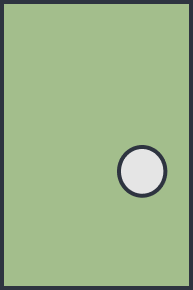
\includegraphics[scale=0.1]{assets/door_sample.png}\\
        \bottomrule
    \end{tabular}
    \caption{The visual representation of symbols in the Ghostless Pacman game}
    \label{tab:1}
\end{table}

Pacman, instead of a a plain `O' might definitely look more like Pacman. In
fact, this Pacman actually munches. Rendering its animation is a feature of the
said SDL library. The same feature allowed the program to display food pieces
as something more delicious than asterisks or any other punctuation, that is,
cherries. The game obstacles that look tougher than `X', and instead of a
dollar sign for the exit door, an exit door.\\

More than these, the resource is also used to render other images such as the
overall interface of the game, including the menus, prompts, and warnings.
Visual assets have been originally constructed using an online software called
\href{https://www.figma.com/}{Figma}.\\

Another use of SDL is for the incorporation of sounds and music into the game.
The audio assets used in the game are royalty-free and, if whose owner demands
copyright, are given proper credit in About the Game.\\

In terms of functions, below are some that have been integrated into the
program as the project requires:

\begin{enumerate}
    \item \codeword{fill_board_with_foods}\\
    \hspace{1em} This function will randomly fill the board with foods
    \item \codeword{fill_board_with_blocks}\\
    \hspace{1em} This function will randomly fill the board with blocks
    \item \codeword{check_if_player_won} and \codeword{check_player_status}\\
    \hspace{1em} These functions work hand-in-hand to check if the player reaches the exit sign after eating all the food pieces,
    or otherwise displays the player status of whether he or she wins or loses
\end{enumerate}

Another crucial function defined is
\codeword{check_for_impossible_win_scenario}, which checks and ensures that any
round in the game is winnable by preventing
\codeword{impassable_adjacent_neighbors}, that is, no food piece or exit door
is surrounded by blocks from all sides.\\

The code also made use of header (.h) files to declare certain variables for
the game. Some major concepts involved are for and while loops, structs, and
switch cases.

\section{Algorithm}
\subsection{Pre-game Algorithm}

\begin{enumerate}
    \item Application launches
    \begin{enumerate}[label=\alph*.]
        \item
            \begin{itemize}[label={}]
                \item If the user presses 1, the \emph{Start} option will be highlighted
                \item \hspace{1cm} If the user presses Enter, proceed to Step 3
            \end{itemize}
        \item 
            \begin{itemize}[label={}]
                \item If the user presses 2, the \emph{Tutorial} option will be highlighted
                \item \hspace{1cm} the user presses Enter, proceed to Step 4
            \end{itemize}
        \item 
            \begin{itemize}[label={}]
                \item  If the user presses 3, the \emph{Exit} option will be highlighted
                \item \hspace{1cm} If the user presses Enter, proceed to Step 5
            \end{itemize}
        \item 
            \begin{itemize}[label={}]
                \item  If the user presses A, the \emph{About the Game} option will be highlighted
                \item \hspace{1cm} If the user presses Enter, proceed to Step 3
            \end{itemize}
        
        \item Else, display a wrong input reminder.
    \end{enumerate}
    
    \item User chooses from the menu options:
        \begin{enumerate}[label=\alph*]
            \item
            \begin{itemize}[label={}]
                \item If the user input is from 2 to 9, display chosen number 
                \item \hspace{1cm} If the user presses Enter, proceed to In-play Algorithm
            \end{itemize}
            \item  If the user presses M, go back to Step 2
	        \item Else, display a wrong input reminder
        \end{enumerate}
    \item User chooses the number of food pieces s/he wants for the game
        \begin{enumerate}[label=\alph*]
            \item User chooses the number of food pieces s/he wants for the game
            \begin{itemize}[label={}]
                \item If the user input is from 2 to 9, display chosen number
            \end{itemize}
            \item If the user presses Enter, proceed to In-play Algorithm
            \item If the user presses M, go back to Step 2
            \item Else, display a wrong input reminder
        \end{enumerate}
    \item Program shows the first slide of the Tutorial
        \begin{enumerate}[label=\alph*]
        \item User navigates through the slides by pressing arrow left (←) and arrow right (→)
        \item If the user presses M, go back to Step 2
        \item If the user presses 1, proceed to Step 3
        \item If the user presses X, proceed to Step 5
        \item Else, display a wrong input reminder
        \end{enumerate}
    \item Program prompts a quit window
        \begin{enumerate}[label=\alph*]
            \item If the user presses Y, exit the program
            \item If the user presses N, the prompt closes
        \end{enumerate}
\end{enumerate}


\subsection{In-game Algorithm}

\begin{enumerate}
    \item Display a 10-by-10 board, with Pacman on the top left, the food
        pieces based on the accepted user input, the randomly distributed
        blocks, and the randomly placed exit door
        \begin{enumerate}[label=\alph*]
            \item If the user presses W, pacman moves up
            \item If the user presses S, pacman moves down
            \item If the user presses A, pacman moves left
            \item If the user presses D, pacman moves right
            \item If the user presses M, the program goes back to menu (go back to Step 2 of the Pre-play Algorithm)
            \item If the user presses X, the program prompts a quit window (recall Step 5 of the Pre-play Algorithm)
            \begin{itemize}[label={}]
                \item If the user presses Y, exit the program
                \item If the user presses N, the prompt closes
            \end{itemize}
        \end{enumerate}
    \item User plays the game by moving Pacman to eat the food pieces towards the exit door
        \begin{enumerate}[label=\alph*]
            \item If Pacman hits a block, display a Game Over prompt
            \item If Pacman gets out of the board, display a Game Over prompt
            \item If Pacman reaches the door without eating all the food pieces, display a Game Over prompt
            \item If Pacman reaches the door after eating all the food pieces, display a Game Victory prompt
        \end{enumerate}
    \item With the prompts from the game results, the user chooses between the options to restart, return to menu, or exit the game
        \begin{enumerate}[label=\alph*]
            \item If the user presses R, restart the game (go back to Step 3 of the Pre-play Algorithm)
            \item If the user presses M, return to menu (go back to Step 2 of the Pre-play Algorithm)
            \item If the user presses X, the program prompts a quit window (recall Step 5 of the Pre-play Algorithm)
                \begin{itemize}[label={}]
                    \item If the user presses Y, exit the program
                    \item If the user presses N, the prompt closes
                \end{itemize}
            \item Else, display a wrong input reminder
        \end{enumerate}
\end{enumerate}


\section{Error handling}

As seen in the algorithms, the game was programmed to handle errors of user input by displaying wrong input reminders per various instances. To recall, below is a list of these occurrences:\\
    \begin{itemize}[label={}]
        \item In Menu, the program displays a reminder when the user keypress is not '1', '2', '3', or 'A'
        \item In the Game
            \begin{itemize}[label={}]
                \item In choosing the food number, the program displays a reminder when the user chooses a number outside the range from 2 to 9
                \item In playing the game, the program displays a reminder when the user presses keys other than 'W', 'S', 'A', or 'D' to move Pacman, and when the user presses keys other than 'M' to return to menu or 'X' to exit the game
                \item In choosing an option after the game results, displayed through the game prompts, the program displays a reminder when the user presses keys other than 'R' to restart, 'M' to return to menu, or 'X' to exit
            \end{itemize}
        \item In Tutorial
            \begin{itemize}[label={}]
                \item In navigating, the program displays a reminder when the user presses keys other than '←' or '→' to navigate through the tutorial slides, when the user presses keys other than 'M' to return to menu
                \item In the last slide, the program displays a reminder when the user presses keys other than '1' to start the game, 'M' to return to menu, or 'X' to exit
            \end{itemize}
        \item In About the Game, the program displays a reminder when the user presses keys other than 'M' to return to menu
    \end{itemize}
\documentclass[11pt]{report}


\usepackage{
        outline,
        pmgraph,
        graphicx,
        verbatim,
        hyperref,
        enumitem,
        float,
        amsmath,
        xcolor,
        listings,
        xparse,
        hyperref
}

\definecolor{codegreen}{rgb}{0,0.6,0}
\definecolor{codegray}{rgb}{0.5,0.5,0.5}
\definecolor{codepurple}{rgb}{0.58,0,0.82}
\definecolor{backcolour}{rgb}{0.95,0.95,0.92}

\lstdefinestyle{mystyle}{
    backgroundcolor=\color{backcolour},   
    commentstyle=\color{codegreen},
    keywordstyle=\color{magenta},
    numberstyle=\tiny\color{codegray},
    stringstyle=\color{codepurple},
    basicstyle=\ttfamily\footnotesize,
    breakatwhitespace=false,         
    breaklines=true,                 
    captionpos=b,                    
    keepspaces=true,                 
    numbersep=5pt,                  
    showspaces=false,                
    showstringspaces=false,
    showtabs=false,                  
    tabsize=2
}

\lstset{style=mystyle}

\NewDocumentCommand{\codeword}{v}{%
    \texttt{\textcolor{black}{#1}}%
}
\setlength{\parindent}{0pt} 

\usepackage[normalem]{ulem}

\title{
    
\includegraphics[width=3in]{upbag.png} \\
    \vspace*{1in}
    \textbf{Machine Project 1}
}


\author{Aaron Paul Gapud\\
        Brymer Bernard Meneses\\
		\vspace*{0.5in} \\
		College of Science\\
        \textbf{University of the Philippines - Baguio}\\
        Gov. Pack Road, Baguio City, Baguio 2600
       } \date{\today}

\setlength{\oddsidemargin}{0in} \setlength{\evensidemargin}{0in}
\setlength{\topmargin}{0in}     \setlength{\headsep}{-.25in}
\setlength{\textwidth}{6.5in}   \setlength{\textheight}{8.5in}

\setlength{\parindent}{0pt}

\renewcommand\thesection{\Alph{section}.} 
\renewcommand\thesubsection{\Roman{subsection}.} 

\date{}

\renewcommand*\contentsname{Table of Contents}

\begin{document}
\maketitle 
\tableofcontents
\newpage

\input{parts/introducion.tex}
\input{parts/description.tex}
\input{parts/algorithm.tex}
\input{parts/error_handling.tex}
\input{parts/manual.tex}
\input{parts/compiling.tex}


\end{document}

\section{Compiling}
\subsection{Windows}

To compile this application, you need to have \textbf{CMake}  and \textbf{GNU
Make} installed your system.  The easiest way to do this is by using the \textbf{scoop
package manager}. \textbf{Scoop} is a package manager for windows that automates the
installation of a plethora of applications through the command line. You can learn more about it
\href{https://github.com/ScoopInstaller/Scoop}{here}.

\subsubsection{Installing Scoop}


To install scoop, open powershell and run the following command:

\begin{lstlisting}[language=bash]
iwr -useb get.scoop.sh | iex
\end{lstlisting}

If you get an error you might need to change the execution policy (i.e. enable Powershell), to do so run the following command and redo the command above.

\begin{lstlisting}[language=bash]
Set-ExecutionPolicy RemoteSigned -scope CurrentUser
\end{lstlisting}

Confirm that you have successfully installed scoop, by running the following command

\begin{lstlisting}[language=bash]
scoop --help
\end{lstlisting}

If the installation was successful, you will be able to see the following:
\begin{lstlisting}
Usage: scoop <command> [<args>]

Some useful commands are:

alias       Manage scoop aliases
bucket      Manage Scoop buckets
cache       Show or clear the download cache
\end{lstlisting}

% \subsubsection{Installing Scoop}
% Once you have successfully installed \textbf{scoop}.
    % excess or kulang?

\subsubsection{Installing CMake and GNU Make}
To install \textbf{CMake} and \textbf{GNU Make} run the following
command:

\begin{lstlisting}[language=bash]
 scoop install cmake make 
\end{lstlisting}
 
To check whether the installation is successful for \textbf{GNU Make} run the following command:

\begin{lstlisting}[language=bash]
make --help
\end{lstlisting}

You will be able to see the following:
\begin{lstlisting}
 Usage: make [options] [target] ...
 Options:
   -b, -m                      Ignored for compatibility.
   -B, --always-make           Unconditionally make all targets.
   -C DIRECTORY, --directory=DIRECTORY
                                   Change to DIRECTORY before doing anything
\end{lstlisting}
    
To check whether the installation is successful for \textbf{CMake} run the following command:

\begin{lstlisting}[language=bash]
cmake --help
\end{lstlisting}

You will be able to see the following:

\begin{lstlisting}[language=bash]
Usage

    cmake [options] <path-to-source>
    cmake [options] <path-to-existing-build>
    cmake [options] -S <path-to-source> -B <path-to-build>

Specify a source directory to (re-)generate a build system for it in the
current working directory.  Specify an existing build directory to
re-generate its build system.
\end{lstlisting}

\subsubsection{Compiling the game}

This project is configured to only work with
the MingGW Compiler, so make sure that it is installed on your computer.\\

Once you have installed \textbf{CMake} and \textbf{GNU Make}, you may now
compile the application. To do so, navigate to the \codeword{ghostless-pacman}
folder and run.
 
\begin{lstlisting}[language=bash]
make build
\end{lstlisting}

This command will automatically download external GUI libraries which were used
in making the game. After that it will compile the program and place it in the
\codeword{bin} folder.

\subsubsection{Running the game}

Now the only thing left is to run the application. You can navigate to the \codeword{bin}
folder and open the \codeword{ghostless-pacman.exe} file which will run the game, or you
can run the following command below to compile and run the application automatically.

\begin{lstlisting}[language=bash]
make run
\end{lstlisting}

Note that, it is important to avoid moving the executable since Windows will not
be able to find the DLLs which are required for running the game.\\

Hooray! You have now compiled and ran the application.

\subsection{Linux}

\subsubsection{Installing the dependencies}

Use your distribution’s package manager to install the following packages:

\begin{itemize}
    \item cmake
    \item make
    \item SDL2
    \item SDL2 Mixer
    \item SDL2 Image
\end{itemize}

\subsubsection{Compiling the source code}
Navigate to the \codeword{ghostless-pacman} folder and run the 
following command.

\begin{lstlisting}[language=bash]
make run
\end{lstlisting}

Hooray! You have now compiled and ran the application.



\end{document}

\section{Compiling}
\subsection{Windows}

To compile this application, you need to have \textbf{CMake}  and \textbf{GNU
Make} installed your system.  The easiest way to do this is by using the \textbf{scoop
package manager}. \textbf{Scoop} is a package manager for windows that automates the
installation of a plethora of applications through the command line. You can learn more about it
\href{https://github.com/ScoopInstaller/Scoop}{here}.

\subsubsection{Installing Scoop}


To install scoop, open powershell and run the following command:

\begin{lstlisting}[language=bash]
iwr -useb get.scoop.sh | iex
\end{lstlisting}

If you get an error you might need to change the execution policy (i.e. enable Powershell), to do so run the following command and redo the command above.

\begin{lstlisting}[language=bash]
Set-ExecutionPolicy RemoteSigned -scope CurrentUser
\end{lstlisting}

Confirm that you have successfully installed scoop, by running the following command

\begin{lstlisting}[language=bash]
scoop --help
\end{lstlisting}

If the installation was successful, you will be able to see the following:
\begin{lstlisting}
Usage: scoop <command> [<args>]

Some useful commands are:

alias       Manage scoop aliases
bucket      Manage Scoop buckets
cache       Show or clear the download cache
\end{lstlisting}

% \subsubsection{Installing Scoop}
% Once you have successfully installed \textbf{scoop}.
    % excess or kulang?

\subsubsection{Installing CMake and GNU Make}
To install \textbf{CMake} and \textbf{GNU Make} run the following
command:

\begin{lstlisting}[language=bash]
 scoop install cmake make 
\end{lstlisting}
 
To check whether the installation is successful for \textbf{GNU Make} run the following command:

\begin{lstlisting}[language=bash]
make --help
\end{lstlisting}

You will be able to see the following:
\begin{lstlisting}
 Usage: make [options] [target] ...
 Options:
   -b, -m                      Ignored for compatibility.
   -B, --always-make           Unconditionally make all targets.
   -C DIRECTORY, --directory=DIRECTORY
                                   Change to DIRECTORY before doing anything
\end{lstlisting}
    
To check whether the installation is successful for \textbf{CMake} run the following command:

\begin{lstlisting}[language=bash]
cmake --help
\end{lstlisting}

You will be able to see the following:

\begin{lstlisting}[language=bash]
Usage

    cmake [options] <path-to-source>
    cmake [options] <path-to-existing-build>
    cmake [options] -S <path-to-source> -B <path-to-build>

Specify a source directory to (re-)generate a build system for it in the
current working directory.  Specify an existing build directory to
re-generate its build system.
\end{lstlisting}

\subsubsection{Compiling the game}

This project is configured to only work with
the MingGW Compiler, so make sure that it is installed on your computer.\\

Once you have installed \textbf{CMake} and \textbf{GNU Make}, you may now
compile the application. To do so, navigate to the \codeword{ghostless-pacman}
folder and run.
 
\begin{lstlisting}[language=bash]
make build
\end{lstlisting}

This command will automatically download external GUI libraries which were used
in making the game. After that it will compile the program and place it in the
\codeword{bin} folder.

\subsubsection{Running the game}

Now the only thing left is to run the application. You can navigate to the \codeword{bin}
folder and open the \codeword{ghostless-pacman.exe} file which will run the game, or you
can run the following command below to compile and run the application automatically.

\begin{lstlisting}[language=bash]
make run
\end{lstlisting}

Note that, it is important to avoid moving the executable since Windows will not
be able to find the DLLs which are required for running the game.\\

Hooray! You have now compiled and ran the application.

\subsection{Linux}

\subsubsection{Installing the dependencies}

Use your distribution’s package manager to install the following packages:

\begin{itemize}
    \item cmake
    \item make
    \item SDL2
    \item SDL2 Mixer
    \item SDL2 Image
\end{itemize}

\subsubsection{Compiling the source code}
Navigate to the \codeword{ghostless-pacman} folder and run the 
following command.

\begin{lstlisting}[language=bash]
make run
\end{lstlisting}

Hooray! You have now compiled and ran the application.



\end{document}

\section{Compiling}
\subsection{Windows}

To compile this application, you need to have \textbf{CMake}  and \textbf{GNU
Make} installed your system.  The easiest way to do this is by using the \textbf{scoop
package manager}. \textbf{Scoop} is a package manager for windows that automates the
installation of a plethora of applications through the command line. You can learn more about it
\href{https://github.com/ScoopInstaller/Scoop}{here}.

\subsubsection{Installing Scoop}


To install scoop, open powershell and run the following command:

\begin{lstlisting}[language=bash]
iwr -useb get.scoop.sh | iex
\end{lstlisting}

If you get an error you might need to change the execution policy (i.e. enable Powershell), to do so run the following command and redo the command above.

\begin{lstlisting}[language=bash]
Set-ExecutionPolicy RemoteSigned -scope CurrentUser
\end{lstlisting}

Confirm that you have successfully installed scoop, by running the following command

\begin{lstlisting}[language=bash]
scoop --help
\end{lstlisting}

If the installation was successful, you will be able to see the following:
\begin{lstlisting}
Usage: scoop <command> [<args>]

Some useful commands are:

alias       Manage scoop aliases
bucket      Manage Scoop buckets
cache       Show or clear the download cache
\end{lstlisting}

% \subsubsection{Installing Scoop}
% Once you have successfully installed \textbf{scoop}.
    % excess or kulang?

\subsubsection{Installing CMake and GNU Make}
To install \textbf{CMake} and \textbf{GNU Make} run the following
command:

\begin{lstlisting}[language=bash]
 scoop install cmake make 
\end{lstlisting}
 
To check whether the installation is successful for \textbf{GNU Make} run the following command:

\begin{lstlisting}[language=bash]
make --help
\end{lstlisting}

You will be able to see the following:
\begin{lstlisting}
 Usage: make [options] [target] ...
 Options:
   -b, -m                      Ignored for compatibility.
   -B, --always-make           Unconditionally make all targets.
   -C DIRECTORY, --directory=DIRECTORY
                                   Change to DIRECTORY before doing anything
\end{lstlisting}
    
To check whether the installation is successful for \textbf{CMake} run the following command:

\begin{lstlisting}[language=bash]
cmake --help
\end{lstlisting}

You will be able to see the following:

\begin{lstlisting}[language=bash]
Usage

    cmake [options] <path-to-source>
    cmake [options] <path-to-existing-build>
    cmake [options] -S <path-to-source> -B <path-to-build>

Specify a source directory to (re-)generate a build system for it in the
current working directory.  Specify an existing build directory to
re-generate its build system.
\end{lstlisting}

\subsubsection{Compiling the game}

This project is configured to only work with
the MingGW Compiler, so make sure that it is installed on your computer.\\

Once you have installed \textbf{CMake} and \textbf{GNU Make}, you may now
compile the application. To do so, navigate to the \codeword{ghostless-pacman}
folder and run.
 
\begin{lstlisting}[language=bash]
make build
\end{lstlisting}

This command will automatically download external GUI libraries which were used
in making the game. After that it will compile the program and place it in the
\codeword{bin} folder.

\subsubsection{Running the game}

Now the only thing left is to run the application. You can navigate to the \codeword{bin}
folder and open the \codeword{ghostless-pacman.exe} file which will run the game, or you
can run the following command below to compile and run the application automatically.

\begin{lstlisting}[language=bash]
make run
\end{lstlisting}

Note that, it is important to avoid moving the executable since Windows will not
be able to find the DLLs which are required for running the game.\\

Hooray! You have now compiled and ran the application.

\subsection{Linux}

\subsubsection{Installing the dependencies}

Use your distribution’s package manager to install the following packages:

\begin{itemize}
    \item cmake
    \item make
    \item SDL2
    \item SDL2 Mixer
    \item SDL2 Image
\end{itemize}

\subsubsection{Compiling the source code}
Navigate to the \codeword{ghostless-pacman} folder and run the 
following command.

\begin{lstlisting}[language=bash]
make run
\end{lstlisting}

Hooray! You have now compiled and ran the application.



\end{document}
